\documentclass{ieeeaccess}
\usepackage{amsmath,amssymb,amsfonts}
\usepackage{graphicx}
\usepackage{textcomp}
\usepackage[utf8]{inputenc}

% BibTeX logo definition according to IEEE Access standard
\def\BibTeX{{\rm B\kern-.05em{\sc i\kern-.025em b}\kern-.08em
    T\kern-.1667em\lower.7ex\hbox{E}\kern-.125emX}}

\usepackage[T1]{fontenc}
\usepackage{lmodern}
\usepackage{mathptmx}

\usepackage{booktabs}
\usepackage{siunitx}

\usepackage{comment}

\usepackage{bm}
\usepackage{algorithm}
\usepackage{algpseudocode}
% Hyperref para criar marcadores (bookmarks) no PDF
\usepackage[
    bookmarks=true,
    bookmarksopen=true,
    bookmarksnumbered=true,
    colorlinks=true,
    linkcolor=blue,
    citecolor=blue,
    urlcolor=blue,
    pdfstartview=FitH,
    pdftitle={Context-oriented Synthesis of Salt Domes in Labeled Seismic Images},
    pdfauthor={Luciano D. Terres, Jacob Scharcanski}
]{hyperref}

%Your document starts from here ___________________________________________________
\begin{document}
\history{Date of publication 2025 12, 0000, date of current version xxxx 00, 0000.}
\doi{10.1109/ACCESS.2024.0429000}

\title{Context-oriented Synthesis of Salt Domes in Labeled Seismic Images}
\author{\uppercase{Luciano D. Terres}\authorrefmark{1} and
\uppercase{Jacob Scharcanski}\authorrefmark{1}, \IEEEmembership{Senior Member, IEEE} }

\address[1]{Institute of Informatics,
Federal University of Rio Grande do Sul, Porto Alegre, RS, Brasil, 91501-970 (e-mail: ldterres@inf.ufrgs.br; jacobs@inf.ufrgs.br)}

\markboth
{Author \headeretal: Preparation of Papers for IEEE TRANSACTIONS and JOURNALS}
{Author \headeretal: Preparation of Papers for IEEE TRANSACTIONS and JOURNALS}

\corresp{Corresponding author: Jacob Scharcanski (e-mail: jacobs@inf.ufrgs.br).}


\begin{abstract}
Advanced remote sensing and seismic image interpretation methods rely on large annotated datasets for training robust machine learning models. However, obtaining such datasets is challenging in applications like offshore oil exploration, where expert annotation is costly and time-consuming. This work proposes a context-oriented data augmentation method for generating synthetic seismic images of salt dome structures with pixel-level mask labels. The proposed approach combines Variational Autoencoders to learn and generate realistic salt body geometries with context-aware non-parametric texture synthesis to create seismic textures across three distinct zones: salt bodies, conventional rocks, and their boundaries. Using the TGS Salt Identification Challenge dataset, we generated synthetic samples that were evaluated by three expert geoscientists and compared against a state-of-the-art method. The qualitative evaluation shows that the synthetic images are virtually indistinguishable from real ones, with expert F1-scores differing by less than 2\%. Furthermore, quantitative comparisons demonstrate substantial improvements over the baseline, achieving significantly lower pixel-wise error, higher structural similarity, and more accurate texture fidelity. These results validate the effectiveness of the proposed context-oriented approach for generating high-quality synthetic seismic training data, which is crucial for seismic interpretation and data augmentation.
\end{abstract}

\begin{keywords}
Data augmentation, deep learning, image segmentation, seismic images, seismic interpretation, texture synthesis, and variational autoencoders.
\end{keywords}

\titlepgskip=-21pt

\maketitle

\section{Introduction}
\label{sec:introduction}
\PARstart{A} relevant task in seismic imaging and interpretation is to distinguish accurately saline bodies from other sediments. However, seismic reflections in salt rocks pose a challenge to seismic imaging researchers due to their distinct acoustic characteristics and complex geometry. The boundaries of saline bodies can be identified by trained experts~\cite{Zeng2019}, but this process involves massive amounts of data and is labor intensive, making it a potential candidate for being handled by smart image segmentation methods. Nevertheless, public databases of annotated seismic images are scarce, and such data is needed for training seismic image segmentation methods based on deep neural networks, such as RESNET~\cite{He2016} and UNET~\cite{Ronneberger2015}, which are specialized in image segmentation and recognition. Therefore, researchers have recently directed their efforts towards data augmentation through seismic image synthesis~\cite{Henriques2021}.

In this work, we propose a mechanism for synthesizing annotated seismic image samples containing salt domes. We use a combination of Variational Autoencoder (VAE) and a context-oriented texture synthesis method to generate new samples. The VAE comprises an encoder that maps the multidimensional input into a low-dimensional latent space, and a decoder that reconstructs the output from these latent features. We aim to minimize the difference between the input and reconstructed samples~\cite{Li2020}.

Visual texture synthesis learns to generate new samples from a particular image by inferring its generation process from examples. The generated textures should be indistinguishable from real data from the human experts' point of view. If experts cannot distinguish between an original texture and a synthesized one, the synthesis process is considered successful~\cite{Gatys2015}. This work innovates by combining VAEs to generate salt and rock shapes with a context-oriented texture synthesis process, which handles non-stationary textures of salt bodies, conventional rocks, and their boundaries. 

\subsection{Organization of the Paper}
The remainder of this paper is organized as follows. Section~\ref{sec:related} reviews the related work in seismic image synthesis and generative models. Section~\ref{sec:background} provides the theoretical background on VAEs, texture synthesis, and seismic image characteristics. Section~\ref{sec:methodology} presents the proposed methodology, detailing the VAE architecture, the texture synthesis approach, and the complete pipeline for generating synthetic seismic images. Section~\ref{sec:results} discusses the experimental setup, evaluation metrics, and results obtained from the proposed method. Finally, Section~\ref{sec:conclusion} concludes the paper and suggests directions for future work.

\section{Related Work}
\label{sec:related}

\PARstart{O}{ver} the past decades, a broad spectrum of algorithms has been proposed to address the challenges in seismic image synthesis. In the early days, before the rise of neural networks, researchers relied on traditional methods like model-based approaches and basic texture synthesis techniques. These methods worked reasonably well for simple tasks but often struggled with complex geological features and non-uniform textures commonly found in seismic data. The primary limitation of these early techniques was their inability to handle non-stationary textures, which are textures that change across different regions of an image~\cite{Zhou2018}.

In recent years, the adoption of deep learning techniques has significantly advanced the field of seismic image synthesis~\cite{Zeng2019}. The introduction of neural networks around 2010 marked a major turning point. Convolutional Neural Networks (CNNs), in particular, brought a new level of sophistication to seismic image synthesis. CNNs excel at extracting detailed features from images, such as horizontal and vertical lines, and can even complete entire objects within an image. This capability allowed for more accurate and realistic seismic images, enabling better interpretation of subsurface structures~\cite{Powers2011}. 

However, the success of CNNs came with a significant challenge: these learning structures require large, annotated datasets for training. In seismic imaging, such datasets tend to be unavailable or difficult to produce. Therefore, researchers have explored various alternatives, including data augmentation with synthetic data and transfer learning. Despite these efforts, the issue of limited training data remains a hurdle in the widespread application of CNNs to seismic image synthesis~\cite{Wang2021}.

More recently, in 2020, R. S. Ferreira et al.~\cite{Ferreira2020} proposed similar work for generating synthetic seismic images. In addition to using expert evaluation, they also evaluated their results using metrics that estimate the distance between synthetic and real images. The article addresses the generation of synthetic seismic images of various geological fields, including geological faults and salt domes. In this sense, we compare our results using the same metrics and methodologies, evaluating the realism of synthetic seismic images when contrasted with real images.

Similarly, Henriques et al.~\cite{Henriques2021} proposed a very similar data augmentation method based on training two generative models to augment the number of samples in a seismic image dataset for the semantic segmentation of salt bodies. However, they perform an indirect evaluation of results, based on the improvement in the performance of segmentation methods based on convolutional neural networks, which could be difficult to use as a direct comparison of results with our proposed method and a different database.

Choi et al.~\cite{Choi2025} address the scarcity of labeled seismic data for training deep learning models by employing advanced generative techniques. They propose a method for generating synthetic seismic images using diffusion models, a class of generative models proficient in various image synthesis tasks. While the primary focus is on generating data for fault detection, their conditional diffusion model incorporates geological context, ensuring the synthetic images are not only realistic but also geologically plausible. The study demonstrates that diffusion models can effectively capture the complex patterns and textures in seismic data, yielding high-quality synthetic images. The results confirm that these synthetic images enhance the training of fault detection algorithms, leading to improved performance in identifying subsurface structures.

In summary, while there has been significant progress in the field of seismic image synthesis, challenges remain in terms of data availability, evaluation methodologies, and the need for more robust generative models. Our work aims to address these challenges by leveraging VAEs and advanced texture synthesis techniques to produce high-quality synthetic seismic images.

\section{Background and Fundamentals}
\label{sec:background}

\PARstart{T}{his} section provides the theoretical foundation for the proposed methodology, introducing the key concepts and techniques that underpin our approach to seismic image synthesis.

\subsection{Variational Autoencoders}

VAEs are deep generative models that learn to encode data into a lower-dimensional latent space and then decode it back to the original space~\cite{Kingma2014}. VAEs are particularly suitable for generating new samples that follow the same distribution as the training data, making them ideal for data augmentation tasks in seismic imaging.

\subsection{Texture Synthesis}

Texture synthesis is a technique used in computer graphics and image processing to generate new textures that are visually similar to a given sample texture. Non-parametric texture synthesis methods~\cite{Efros1999} create new images by sampling and recombining patches from example textures, ensuring that the statistical properties of the generated texture match those of the original.

\subsection{Seismic Image Characteristics}

Seismic images present unique challenges due to their non-stationary nature, where texture patterns vary significantly across different geological structures. Salt bodies, in particular, exhibit distinct acoustic properties that create characteristic boundary patterns in seismic data. Understanding these characteristics is essential for developing effective synthesis methods that can generate realistic seismic images.

\section{Proposed Methodology}
\label{sec:methodology}

\subsection{Overview of the Approach}

\PARstart{T}{he} Context-Oriented Seismic Image Synthesis methodology combines a deep learning model based on a VAE with a texture synthesis algorithm. It generates seismic image samples for data augmentation within a specific context mask. The proposed approach consists of two main stages: (1) context generation using a VAE that generates salt body masks corresponding to a given salt geometry, and (2) texture synthesis using a non-parametric algorithm that creates realistic seismic images based on the generated masks. The proposed method focuses on context zones and on the characteristics of seismic images with salt domes, ensuring that the synthetic samples preserve the structural and textural properties of real seismic data. Figure~\ref{fig:synthesis_pipeline} illustrates the complete synthesis pipeline, showing how the VAE-generated masks are combined with context-oriented texture synthesis to produce realistic synthetic seismic images.

\begin{figure}[htbp]
    \centering
    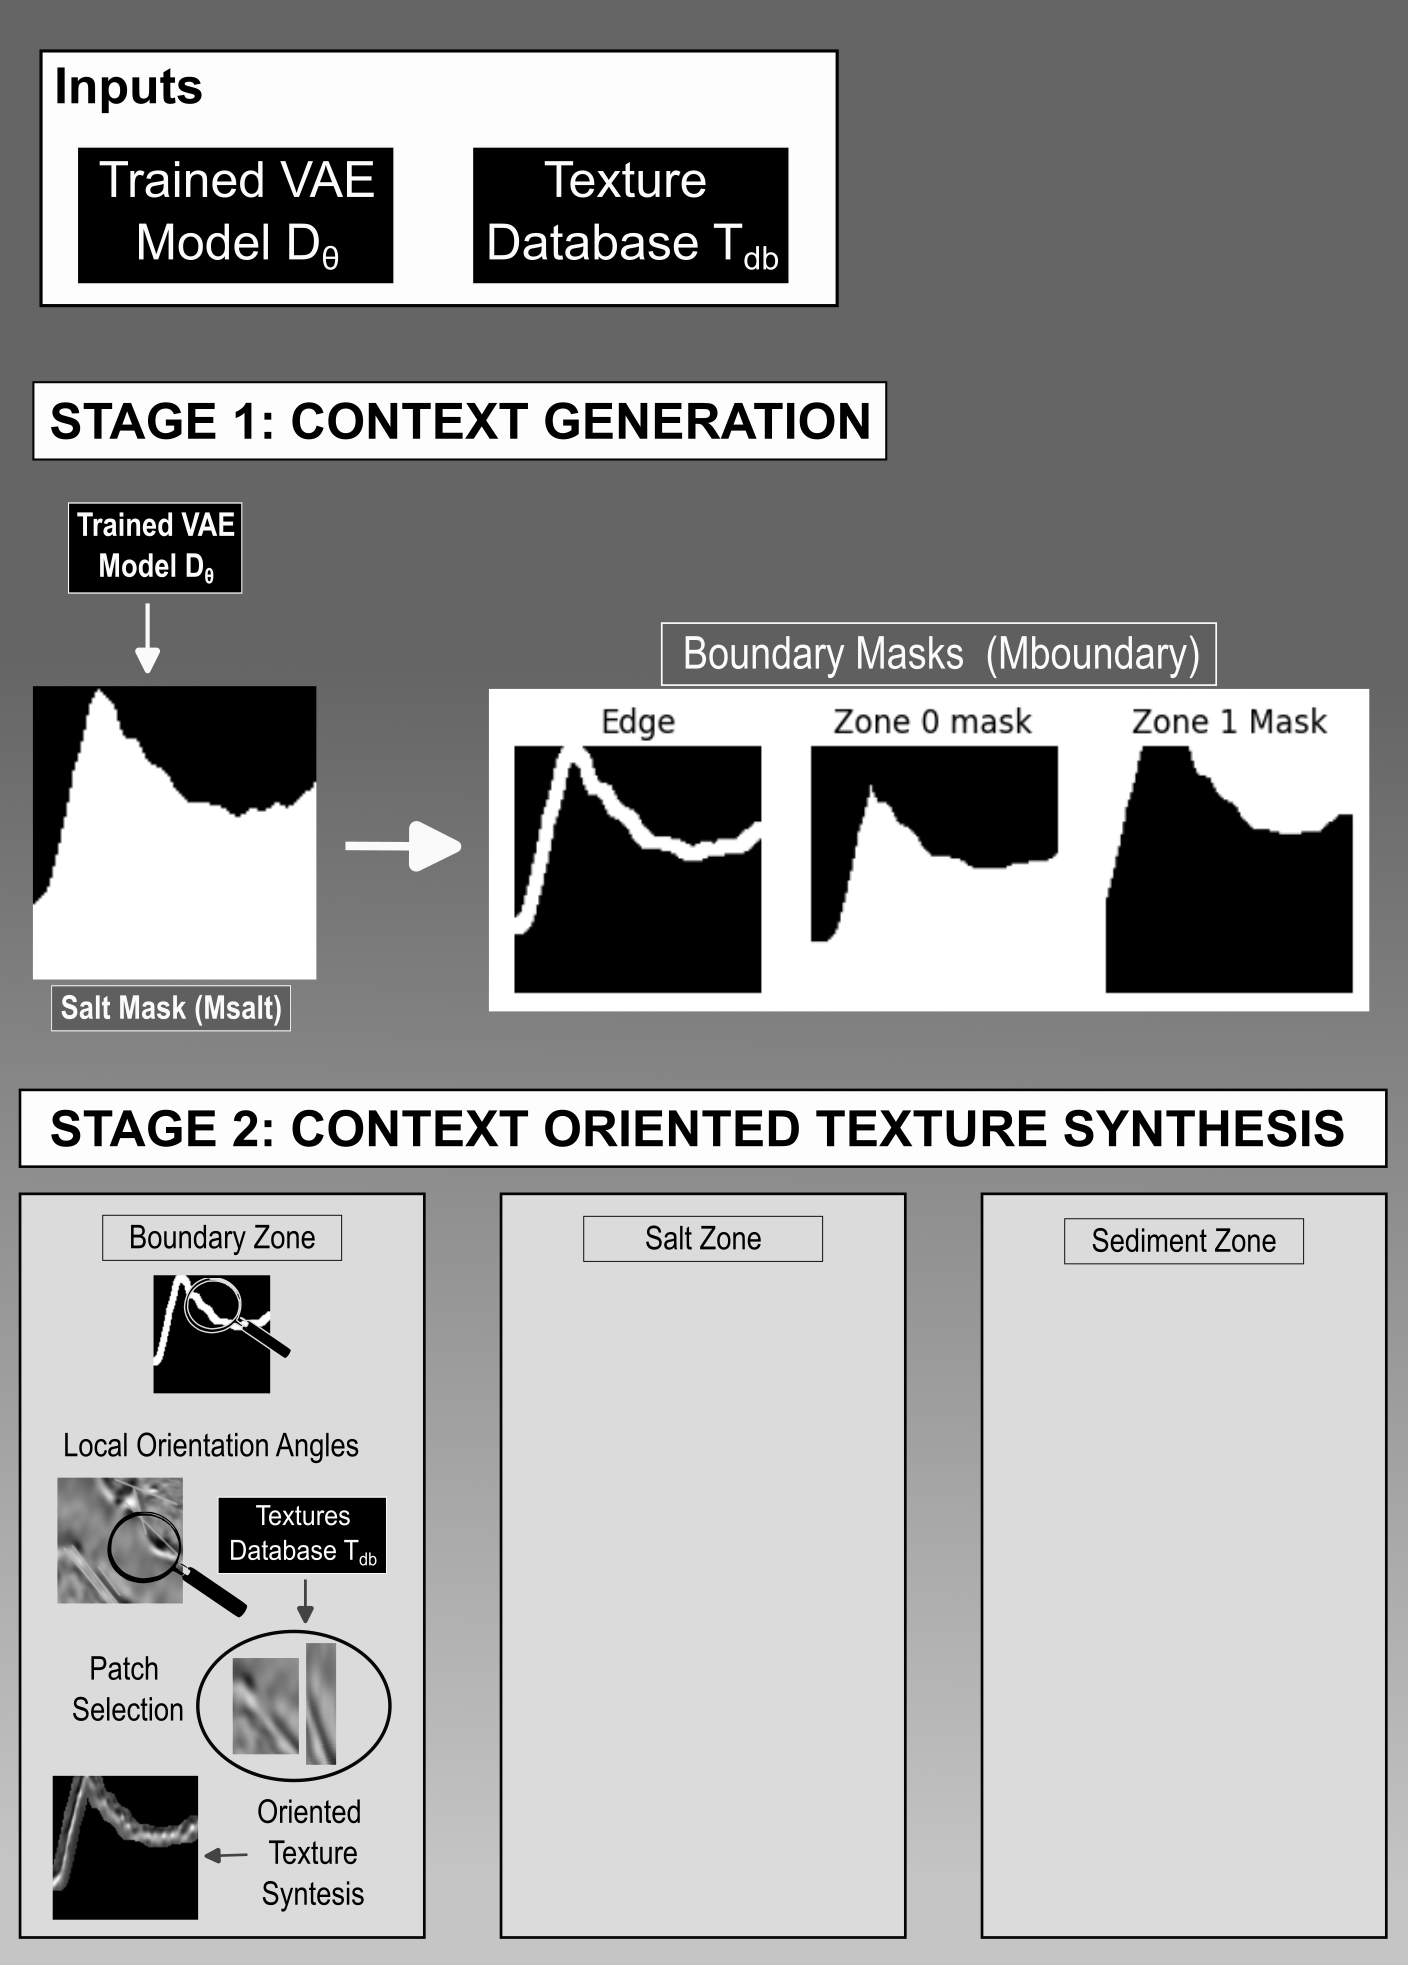
\includegraphics[width=1\linewidth]{images/g50.png}
    \caption{Complete pipeline of the proposed context-oriented seismic image synthesis methodology, showing the integration of VAE-based mask generation and context-aware texture synthesis.}
    \label{fig:synthesis_pipeline}
\end{figure}

\subsection{Context Generation Using a Variational Autoencoder}

The proposed data augmentation scheme detects and generates new rock geometries with a VAE, as shown in Fig.~\ref{fig:vae1}.  
\begin{figure}[htbp]
    \centering
    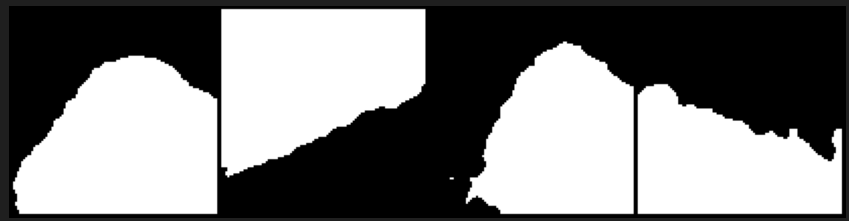
\includegraphics[width=1\linewidth]{images/vaesGen.png}
    \caption{Samples of generated structural salt masks. The Variational Autoencoder learns the distribution and reproduce new structural masks.}
    \label{fig:vae1}
\end{figure}

Fig.~\ref{fig:vae1} illustrates a dataset of seismic images used to generate new salt masks. The natural intersection between two different rocks are their boundaries, and in the case of salt rock this boundary is usually apparent, as Fig.~\ref{fig:edge1} shows. During the VAE training process, we use only salt masks with a considerable amount of salt, varying from 10 to 90 percent of the total area.
\begin{figure}[htbp]
    \centering
    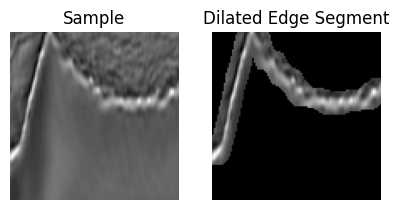
\includegraphics[width=1\linewidth]{images/edge detection.png}
    \caption{Sample of the boundaries identification between salt and other sediments represented in a dilated edge segment.}
    \label{fig:edge1}
\end{figure}

We use the generated masks as contexts for the texture synthesis process. Once we know the boundaries of a salt body, we expect the interior region to be salt. The VAE model we use in this work employs a simple feedforward network for the encoder and decoder. The encoder contains four stacked dense layers, and the decoder contains five stacked dense layers. During inference, we sample the latent variables $z$ from the prior distribution $\pi(z)$, and then decode $z$ with the VAE's decoder to generate the salt mask with the inferred distribution.

The main task of VAEs is to model the underlying probability distribution of a data set $\bm{x} = \{x^{(1)}, x^{(2)}, \ldots, x^{(N)}\}$, where each $x^{(i)}$ represents an individual sample. The model introduces a latent variable $\bm{z}$ (a lower-dimensional representation) and parameters $\theta$ to maximize the marginal likelihood $p_\theta(x)$, where $x$ is the observed data:

\begin{equation}
p_\theta(x) = \int p_\theta(x | z) p(z) \, dz
\end{equation}
where $p_\theta(x | z)$ is the likelihood of $x$ given $z$, and $p(z)$ is the prior distribution over the latent variables.

The key VAE components are the following:

\paragraph{Encoder (Recognition Model)}
Maps an input $x$ to a latent variable $z$, and approximates the posterior distribution $q_\phi(z | x)$ (parameterized by $\phi$) assuming it is Gaussian:

\begin{equation}
q_\phi(z | x) = \mathcal{N}(z; \mu_\phi(x), \Sigma_\phi(x))
\end{equation}
where $\mu_\phi(x)$ and $\Sigma_\phi(x)$ are the mean and covariance of the posterior distribution $q_\phi(z | x)$, which are outputs of the encoder network.

\paragraph{Decoder (Generative Model)}
Reconstructs the data from the latent variable $z$, modeling the likelihood $p_\theta(x | z)$ (parameterized by $\theta$) assuming it as Gaussian:

\begin{equation}
p_\theta(x | z) = \mathcal{N}(x; \mu_\theta(z), \Sigma_\theta(z))
\end{equation}

where $\mu_\theta(z)$ and $\Sigma_\theta(z)$ are the mean and covariance of the likelihood distribution, which are outputs of the decoder network.

\paragraph{Latent Variables Priors $p(z)$}
Usually assumed as a standard normal distribution:

\begin{equation}
p(z) = \mathcal{N}(z; 0, \mathrm{I})
\end{equation}

where $\mathrm{I}$ is the identity matrix.

\paragraph{Variational Inference} Since the exact posterior $p(z | x)$ is intractable, VAEs use variational inference to approximate it by optimizing the evidence lower bound (ELBO), where $\text{KL}(\cdot \parallel \cdot)$ denotes the Kullback-Leibler divergence:

\begin{equation}
\log p_\theta(x) \geq \mathbb{E}_{q_\phi(z | x)} \left[ \log p_\theta(x | z) \right] - \text{KL}(q_\phi(z | x) \parallel p(z)),
\end{equation}
and the ELBO has two important components: reconstruction loss and Kullback-Leibler (KL) divergence loss, which are detailed next. The reconstruction loss is the expected log-likelihood of the data, which encourages accurate sample reconstruction:

\begin{equation}
\mathbb{E}_{q_\phi(z | x)} \left[ \log p_\theta(x | z) \right]
\end{equation}
and the KL divergence loss is the Kullback-Leibler divergence between the approximate posterior and the prior, which acts as a regularizer. For Gaussian distributions, this can be computed in closed form as:

\begin{equation}
\begin{aligned}
\text{KL}(q_\phi(z | x) \parallel p(z))
=  \\
\frac{1}{2} \sum_{i=1}^{d} \left( \mu_\phi(x)_i^2 + \Sigma_\phi(x)_{ii} - \log \Sigma_\phi(x)_{ii} - 1 \right)
\end{aligned}
\end{equation}

where $d$ is the dimensionality of the latent space, and $\mu_\phi(x)_i$ and $\Sigma_\phi(x)_{ii}$ denote the $i$-th component of the mean vector and the $i$-th diagonal element of the covariance matrix, respectively.

To enable gradient-based optimization, we use the reparameterization trick. Instead of sampling $z \sim q_\phi(z | x)$ directly, we express $z$ as:

\begin{equation}
z = \mu_\phi(x) + \Sigma_\phi(x)^{1/2} \odot \epsilon, \quad \epsilon \sim \mathcal{N}(0, \mathrm{I})
\end{equation}
where $\epsilon$ is an auxiliary random variable sampled from a standard normal distribution, and $\odot$ denotes element-wise multiplication. This formulation allows gradients to be propagated through $\mu_\phi(x)$ and $\Sigma_\phi(x)$.

Finally, we train VAEs by maximizing the ELBO with respect to the parameters $\theta$ and $\phi$ using stochastic gradient descent. The optimization process balances reconstruction accuracy with latent space regularization.

\subsubsection{Advantages of Variational Autoencoders}
The primary reasons for using VAEs are a realistic generation of synthetic samples, an increase in dataset diversity, a regularization and control of variability, and an improvement in the generalization of the segmentation model. Considering specific reasons related to the nature of seismic data and the purpose of sample generation for data augmentation, VAEs enable the generation of synthetic images that preserve the structural characteristics of real seismic data, thereby enhancing the training and performance of segmentation models~\cite{Henriques2021,Wang2021,Anjom2024}.

\subsubsection{Comparison with Generative Adversarial Networks (GANs)}

\begin{enumerate}
    \item \textbf{Control over Data Variability}:
    \begin{itemize}
        \item It is essential that the generated images preserve the structural patterns of salt bodies. VAEs ensure that synthetic images fall within the expected distribution of real seismic images. GANs, on the other hand, are more prone to generating images with high variability and may occasionally create unrealistic or inconsistent samples~\cite{Zhou2018}.
    \end{itemize}
    \item \textbf{Regularization and Smoothness in Image Generation}:
    \begin{itemize}
        \item VAEs impose a probabilistic structure on the latent space, resulting in smoother transitions between different samples and generating images that maintain coherent structural characteristics. GANs, in turn, can suffer from mode collapse~\cite{Zhou2018}, where they generate only a limited subset of possible data variations, reducing the diversity of the augmented dataset.
    \end{itemize}
    \item \textbf{Training Stability}:
    \begin{itemize}
        \item GANs require a balance between the generator and discriminator, which can make training unstable and more challenging to converge to a distribution that well represents the seismic data~\cite{Zhou2018}.
    \end{itemize}
\end{enumerate}

Although GANs are known for generating high-quality images, we chose VAEs in this work due to their more refined control over data variability, training stability, and preservation of the latent seismic data distribution.

\subsubsection{Disadvantages of Diffusion Models}
Conversely, diffusion models present practical and conceptual disadvantages~\cite{Zhou2024}:
\begin{enumerate}
    \item \textbf{Higher Computational Cost}:
    \begin{itemize}
        \item Diffusion models require many sampling steps to generate images, typically hundreds or thousands of denoising steps~\cite{Zhou2024}. This makes them more computationally expensive than VAEs, which generate samples in a single pass through the model.
        \item In seismic applications, where there is a need to generate a large number of samples for data augmentation, the efficiency of VAEs can be a significant advantage. 
    \end{itemize}
    \item \textbf{Need for Large Volume of Training Data}:
    \begin{itemize}
        \item Diffusion models often require large training datasets to capture high-quality distributions~\cite{Zhou2024}. Since labeled seismic images can be limited, VAEs may be more effective in learning useful representations even with a smaller number of samples.
    \end{itemize}
\end{enumerate}

Therefore, targeting efficiency and ease of training, VAEs have simpler and more stable training, as they do not rely on an iterative refinement process like diffusion models. This can be a decisive factor when there are time and computational resource constraints.

\subsection{Context-oriented Texture Synthesis}

The typical texture synthesis algorithms use an image database and replicate the images in a picture plane according to some arrangement rules. The texture synthesis can be enhanced by working at a finer scale, from the pixel level to a small region level. At each iteration of the algorithm, a small section of the original texture, a patch, is copied and placed within the newly synthesized texture. Non-parametric sampling~\cite{Efros1999} improved further texture synthesis by creating a new image that shares the same statistical properties as a given sample texture, while avoiding explicit models of the texture by directly sampling from example images.

\subsubsection{Non-Parametric Texture Synthesis Algorithm}

The proposed seismic texture synthesis method requires the following components:

\textbf{1. Neighborhood Definition:} For each pixel $p$ in the image to be synthesized, a region around $p$ already filled with known values is defined (namely, a neighborhood $N(p)$);

\textbf{2. Similarity Criterion:} To find corresponding patches in the example image, we compute the similarity between $N(p)$ and the neighborhoods $N(q)$ for all pixels $q$ in the example image. We define a similarity measure as the Euclidean distance $D$ between the pixels of the neighborhoods:

\begin{equation}
D(N(p), N(q)) = \sum_{i \in N} \left( I_p(i) - I_q(i) \right)^2,
\end{equation}
where $I_p(i)$ and $I_q(i)$ are the pixel intensity values at location $i$ in the neighborhoods of pixels $p$ and $q$, respectively, and $N$ denotes the set of pixel locations in the neighborhood;

\textbf{3. Random Sampling:} We choose a pixel $q$ randomly from the example image with probability proportional to its similarity (or inverse of $D(N(p), N(q))$) to $p$. In other words, pixels with smaller distance $D(N(p), N(q))$ are more likely to be chosen. We can model the probability $P(q)$ of selecting pixel $q$ as:

\begin{equation}
P(q) = \frac{\exp(-D(N(p), N(q)) / \sigma^2)}{\sum_{q'} \exp(-D(N(p), N(q')) / \sigma^2)}
\end{equation}
where $\sigma$ is a temperature parameter that controls the influence of distances on the pixel selection probability, and $q'$ denotes all candidate pixels in the example image;

\textbf{4. Image Filling:} The process begins with a small initial patch in the new image and gradually expands it, pixel by pixel, using the steps described above to fill the entire image. The choice of the next pixel to be synthesized follows a raster or spiral filling path. The method produces seismic textures that are visually similar to the original input texture. 

\subsubsection{Context-based Seismic Image Synthesis}

We base the process of seismic image synthesis on the context masks generated by the VAE model. We use various patches as inputs, corresponding to different parts of the seismic image. The synthesized sample has three main components, namely, salt zone, boundary zone, and conventional rock zone. Initially, we create the boundary, or frontier, zones between the two rocks, which we also call edge zone. We create the boundary zone by using edge detection to identify the interface between the two types of rocks, and make it thicker, creating an edge strip. As Fig.~\ref{fig:edge1} shows, this strip is an area of high seismic contrast appearing as light and dark bands. Also, various parallel lines make up this boundary, and Fig.~\ref{fig:line1} shows their angles. We use a dataset composed of edge pieces and their corresponding angles as input for the boundary synthesis process. Then, for each edge segment in the mask of the image to be synthesized, we synthesize its texture based on the patch with the most similar angle (see Fig.~\ref{fig:edge2}). We repeat this process until all the segments of the edge band are covered.

\begin{figure}[htbp]
    \centering
    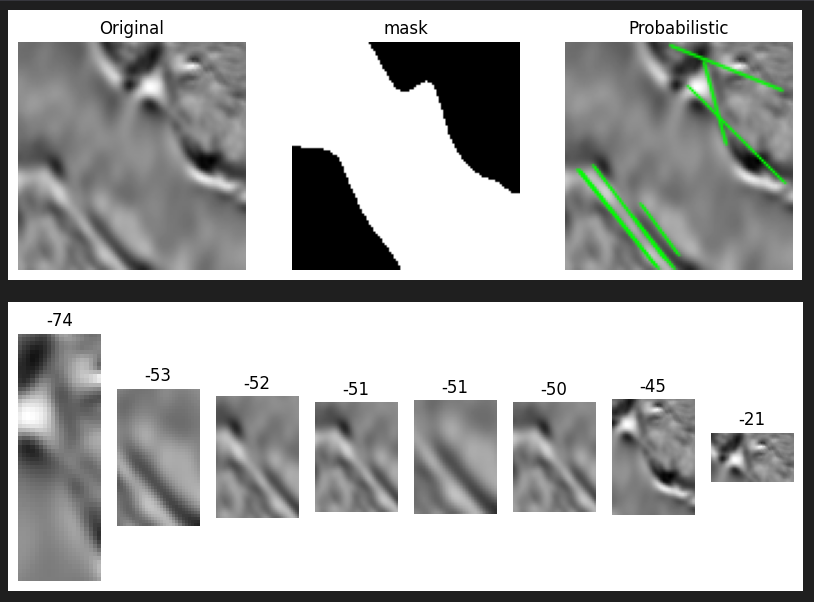
\includegraphics[width=1\linewidth]{images/7.png}
    \caption{The Green lines at original image identify border zones and angles to orient the patch selection for patch database construction process.}
    \label{fig:line1}
\end{figure}

\begin{figure}[htbp]
        \centering
        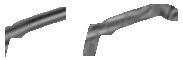
\includegraphics[width=1\linewidth]{images/edge3.jpg}
        \caption{The Construction of new boundaries in generated images uses texture synthesis over selected samples from patch database.}
        \label{fig:edge2}
    \end{figure}    

To synthesize the salt zones, we use the corresponding source image region as a seismic texture reference to generate new synthesized pixels. Finally, we synthesize the conventional rock zone using the corresponding sediment regions in the source sample. We divide the seismic image synthesis into steps to conform to the specific characteristics of this kind of image, such as the edge, saline rock, and conventional rock zones, as Fig.~\ref{fig:source1} shows.

\begin{figure}[htbp]
    \centering
    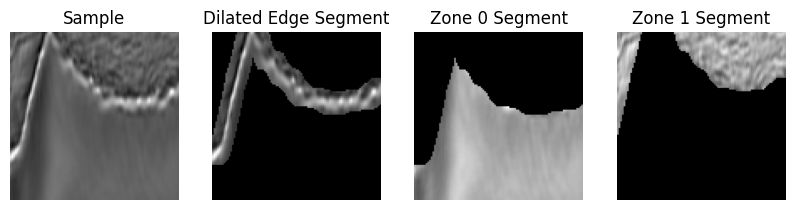
\includegraphics[width=1\linewidth]{images/2.png}
    \caption{Real seismic saline images divided by context zones as input to the texture synthesis process.}
    \label{fig:source1}
\end{figure}

\subsection{Complete Synthesis Pipeline}

The complete synthesis pipeline integrates both the VAE-based context generation and the context-oriented texture synthesis. The algorithm processes all zones, one by one, to complete the seismic image synthesis process using their corresponding zone samples in the input data. The pipeline can be summarized as follows: (1) the VAE generates a new salt body mask defining the geometric structure, (2) edge detection identifies boundary zones between salt and sediment, (3) the texture synthesis algorithm fills each zone (edges, salt, and sediment) with appropriate textures from the training database, and (4) the final synthetic seismic image is assembled by combining all synthesized zones. This systematic approach, detailed in Algorithm~\ref{alg:synthesis}, ensures that the generated images maintain both structural consistency and textural realism.

\begin{algorithm}[htbp]
\caption{Context-Oriented Seismic Image Synthesis}
\label{alg:synthesis}
\begin{algorithmic}[1]
\State \textbf{Input:} Trained VAE model $D_\theta$, Texture Database $T_{db}$
\State \textbf{Output:} Synthetic Seismic Image $I_{synth}$

\vspace{0.2cm}
\Statex \textit{// Stage 1: Context Generation}
\State Sample latent vector $z \sim \mathcal{N}(0, I)$
\State Generate salt mask $M_{salt} \leftarrow D_\theta(z)$
\State Identify boundary mask $M_{boundary}$ from $M_{salt}$ via edge detection and dilation
\State Define sediment mask $M_{sediment} \leftarrow \neg(M_{salt} \cup M_{boundary})$
\State Initialize $I_{synth}$ as an empty image

\vspace{0.2cm}
\Statex \textit{// Stage 2: Context-Oriented Texture Synthesis}
\State \textit{// Synthesize Boundary Zone}
\For{each segment $s$ in $M_{boundary}$}
    \State Compute local orientation $\alpha_s$
    \State Select best patch $P_{boundary} \in T_{db}$ based on $\alpha_s$
    \State Synthesize texture for $s$ in $I_{synth}$ using $P_{boundary}$
\EndFor

\State \textit{// Synthesize Salt Zone}
\State Select salt patches $P_{salt} \in T_{db}$
\State Synthesize texture for region $M_{salt}$ in $I_{synth}$ using $P_{salt}$

\State \textit{// Synthesize Sediment Zone}
\State Select sediment patches $P_{sediment} \in T_{db}$
\State Synthesize texture for region $M_{sediment}$ in $I_{synth}$ using $P_{sediment}$

\vspace{0.2cm}
\State \Return $I_{synth}$
\end{algorithmic}
\end{algorithm}


\section{Results and Discussion}
\label{sec:results}

\PARstart{T}{his} section presents comprehensive experimental results that validate the effectiveness of the proposed approach. The evaluation encompasses both qualitative assessment by domain experts and quantitative comparison with state-of-the-art methods. This dual evaluation strategy demonstrates the model's performance through the following criteria:

\begin{enumerate}
    \item \textbf{Qualitative Evaluation by Experts}: Experts try to identify the portions of salt dome structures inside the seismic samples. The expert produces a mask label that will be compared with the ground truth mask. Quantitative metrics, such as the F1 score, are used to evaluate the difference between the expert prediction and the ground truth. 
    
    \item \textbf{Quantitative Comparison with Related Work}:
    A very similar work In “Generating Sketch-Based Synthetic Seismic Images With Generative Adversarial Networks” \cite{Ferreira2020}, use the metrics mean squared error (MSE), structural similarity (SSIM) and Euclidean distance based on the Local Binary Pattern (LBP) to measure texture attributes between original seismic and the samples synthesized oriented by sketches produced by the networks. We will evaluate the samples generated by our proposed method with the same metrics and compare the results.
\end{enumerate}

\subsection{Dataset}

We obtained the salt body dataset from the TGS Salt Identification Challenge, a machine learning competition on Kaggle. It comprises 2D image slices representing a 3D view of the Earth's interior obtained through reflection seismology. The data is a set of images chosen randomly in the subsurface. The photos are 101 x 101 pixels and each pixel is classified as either salt or sediment \cite{TGS2023}.

\begin{figure}[htbp]
    \centering
    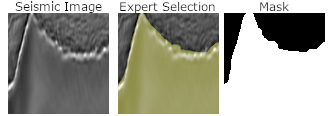
\includegraphics[width=1\linewidth]{images/fig8.png}
    \caption{Comparison between real sample, geoscience specialist selection over saline area and ground truth (saline mask).}
    \label{fig:expert1}
\end{figure}



\subsection{Evaluation Metrics}

Through qualitative analysis, the geoscience specialist evaluates the samples to identify the portions of salt bodies in the seismic images. To assess the quality of generation , the metrics precision, recall, and F1-score compare the synthetic seismic image with the ground truth, as detailed below:

The F1 score is a widely used measure for evaluating binary classification models. It is particularly useful when a balance between precision and recall is desired. It allows access to the quality of the classification predictions. While the correct classification rate is simple to understand, it can be misleading in imbalanced datasets. Therefore, measures such as precision, recall, and the F1 score tend to provide a clearer scenario~\cite{Powers2011}.

\begin{itemize}
    \item \textbf{Precision:} is the proportion of true positives (TP) over all predicted positive results (TP + FP).
    \begin{equation}
    \text{Precision} = \frac{TP}{TP + FP}
    \end{equation}

    \item \textbf{Recall:} or sensitivity, is the proportion of true positives over all actual positive cases (TP + FN).
    \begin{equation}
    \text{Recall} = \frac{TP}{TP + FN}
    \end{equation}


    \item \textbf{F1 Score:} is the harmonic mean of precision and recall, providing a single metric that considers both. 

\end{itemize}
    \begin{equation}
    \text{F1 Score} = 2 \times \frac{\text{Precision} \times \text{Recall}}{\text{Precision} + \text{Recall}}
    \end{equation}
    
 The F1 score is particularly valuable in classification situations where the positive class is rare. It helps to understand the trade-off between false positives and false negatives. In several practical applications, the F1 score provides a balanced measure that is less susceptible to class distribution bias.

We use the precision, recall, and F1-score measures to evaluate the salt bodies masks generated by the experts, and we can compute them using the confusion matrix derived from these expert-generated masks. To evaluate the quality of the synthesized samples, we evaluate the overlap between the experts' selections of pixels corresponding to the salt bodies in synthetic images and synthetic images masks, as Fig.~\ref{fig:expert1} shows.

Fig.~\ref{fig:expert2} illustrates the ground truth image and the specialist evaluation of the salt bodies locations, and the computed precision, recall, and F1-score measures for this particular case.

Regarding quantitative comparison, following the methodology of Ferreira et al.~\cite{Ferreira2020}, we assess the quality of the produced samples by comparing each synthetic image with the original seismic image that serves as a template. The template is the basis for producing the sketches, as shown in Figure~\ref{fig:sketches}, which guide the samples' production. To this end, we use the metrics mean squared error (MSE), Structural Similarity Index (SSIM), and Euclidean distance based on the Local Binary Pattern (LBP) texture attribute between the original template image and the synthetic images.

\begin{figure}[htbp]
	\centering
	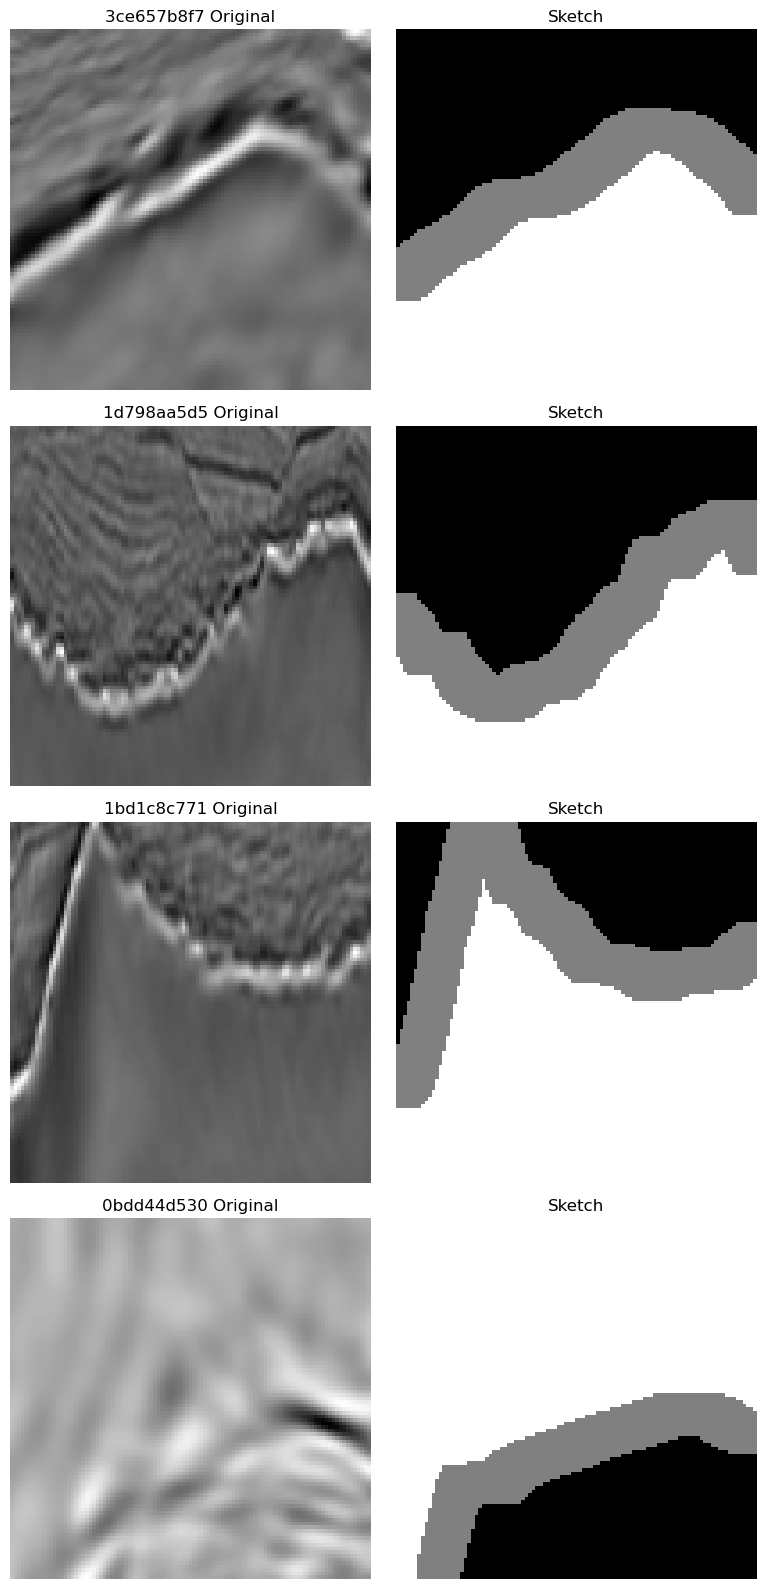
\includegraphics[width=1\linewidth]{images/sketches}
	\caption{Image Sketches based on Original Seismic Templates}
	\label{fig:sketches}
\end{figure}

The MSE defines a pixel-to-pixel distance between two images. We calculate it as follows: subtract each synthetic pixel value from the real one, square each error (this eliminates negative signs and penalizes larger errors), and finally take the average of these squares:

\begin{equation}
\label{eq:mse}
\text{MSE} = \frac{1}{n} \sum_{i=1}^{n} (y_i - \hat{y}_i)^2
\end{equation}

where $n$ is the total number of pixels, $y_i$ is the $i$-th pixel value in the original image, and $\hat{y}_i$ is the corresponding pixel value in the synthetic image.

The SSIM is a metric that measures the perceptual similarity between two images $x$ and $y$ by incorporating texture information, such as variances and covariances. It is widely used in computer vision and image processing to assess the quality of image reconstructions, compressions, or transmissions. It evaluates luminance (brightness), contrast, and structural attributes as local patterns and shapes. Since SSIM values are defined in the range $[-1, 1]$, the common transformation (2) represents it as a distance to facilitate comparison, and from now on, it is called DSSIM:

\begin{equation}
\label{eq:mse2}
\text{DSSIM}(x, y) = \frac{1 - \text{SSIM}(x, y)}{2}
\end{equation}

The interpretation of DSSIM values as a distance between 0 and 1 is as follows: 

\begin{itemize}
    \item DSSIM = 0: the images are identical
    \item DSSIM from 0.005 to 0.10: high similarity
    \item DSSIM > 0.25: low perceptual similarity
    \item DSSIM from 0.5 to 1: very different
\end{itemize}

The LBP is a more robust texture attribute successfully applied in medical images and geosciences \cite{Vatamanu2013,BrittoMattos2017}. The LBP calculation here uses four neighbors, distance 1, and a 64-pixel tile size. The calculation produces a histogram for each image, representing the frequency of local binary patterns. Finally, we compute the Euclidean Distance between the histograms. Therefore, the smaller the distance, the more similar the textures of the two images are. Otherwise, larger histogram distances represent different patterns.

\begin{figure*}[htbp]
    \centering
    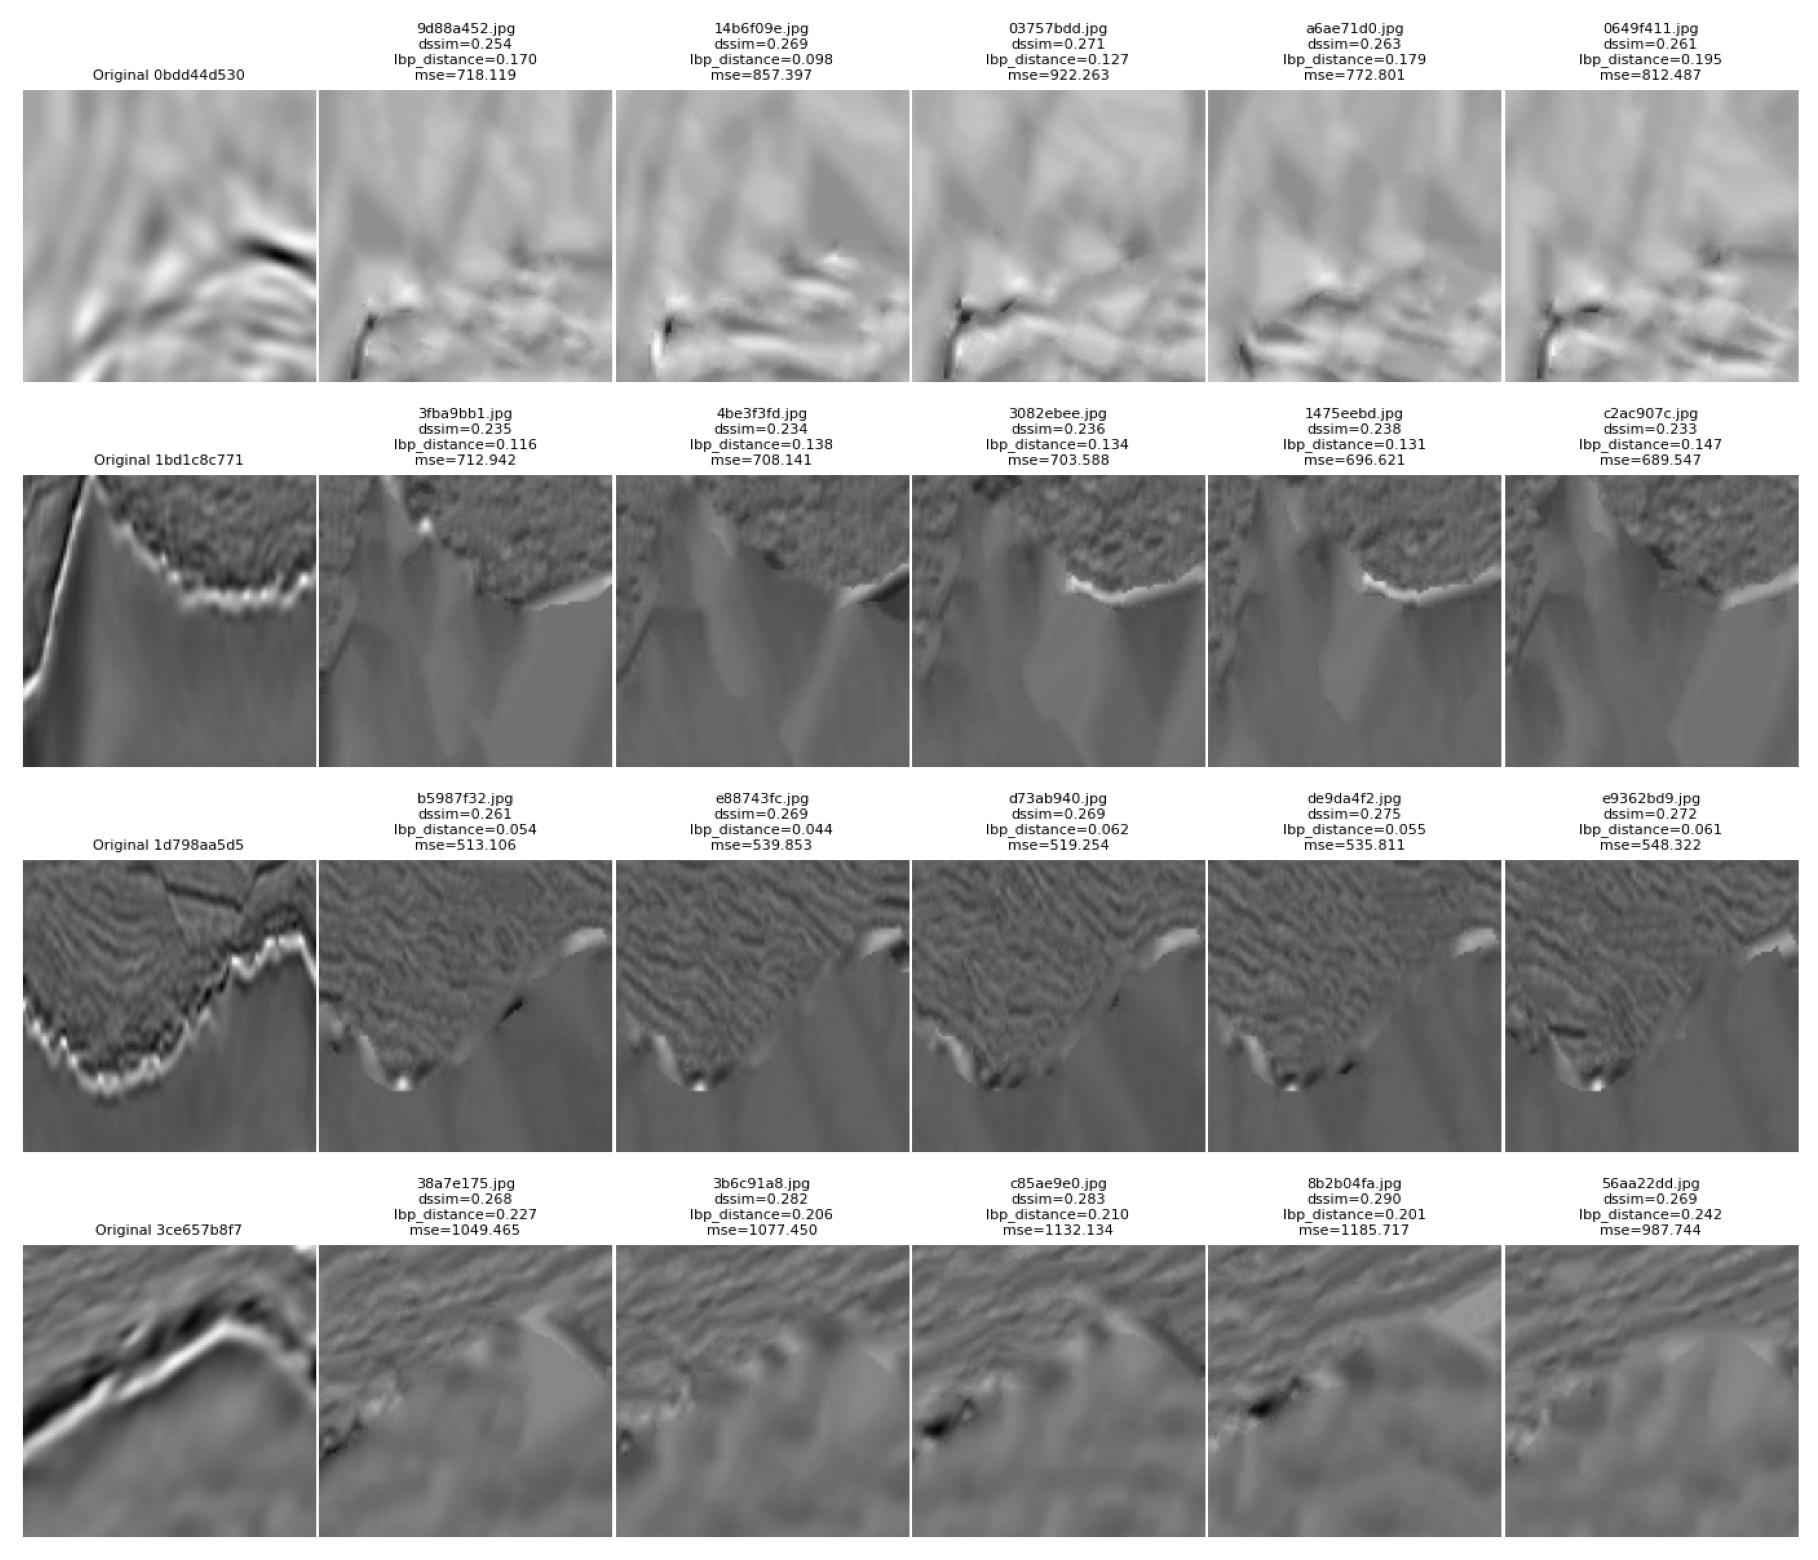
\includegraphics[width=1\textwidth]{images/imagens2.png}
    \caption{Synthetic Seismic Samples}
    \label{fig:placeholder}
\end{figure*}


\begin{figure}[htbp]
    \centering
    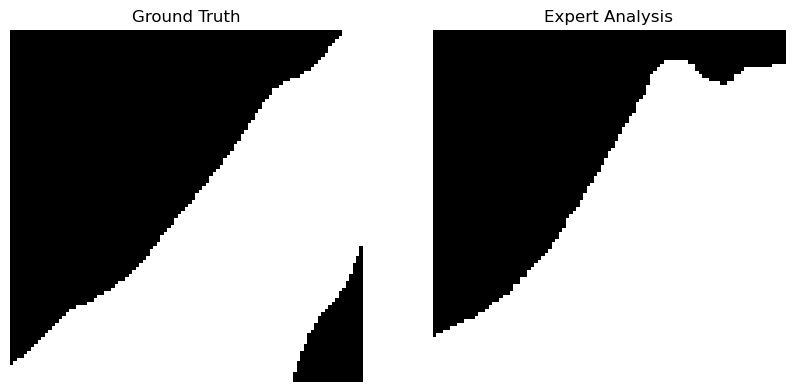
\includegraphics[width=1\linewidth]{images/expert.png}
    \caption{Quantitative analysis demonstration: Sample measurement between ground truth and expert analysis: Precision: 0.88 ; Recall: 0.87 ; F1-score: 0.87.}
    \label{fig:expert2}
\end{figure}

\begin{table*}[htbp]
\centering
\caption{Result table: real images evaluation by the experts.}
\label{tab:real_images_evaluation}
\sisetup{output-decimal-marker = {,}}
\begin{tabular*}{\textwidth}{@{\extracolsep{\fill}}l S[table-format=1.5] S[table-format=1.5] S[table-format=1.5] S[table-format=1.5] S[table-format=1.5] S[table-format=1.5] S[table-format=1.5] S[table-format=1.5] S[table-format=1.5] S[table-format=1.5]@{}}
\toprule
& \multicolumn{3}{c}{\textbf{Expert 1}} & \multicolumn{3}{c}{\textbf{Expert 2}} & \multicolumn{3}{c}{\textbf{Expert 3}} & \textbf{Mean} \\
\cmidrule(lr){2-4} \cmidrule(lr){5-7} \cmidrule(lr){8-10}
\textbf{Metrics} & {\textbf{Precision}} & {\textbf{Recall}} & {\textbf{F1-score}} & {\textbf{Precision}} & {\textbf{Recall}} & {\textbf{F1-score}} & {\textbf{Precision}} & {\textbf{Recall}} & {\textbf{F1-score}} & {\textbf{F1-score}} \\
\midrule
Std Dev & 0.06034 & 0.04584 & 0.04037 & 0.05429 & 0.04763 & 0.04408 & 0.04780 & 0.05288 & 0.03414 & 0.03953 \\
Mean & 0.91480 & 0.91563 & 0.91396 & 0.91845 & 0.90420 & 0.91064 & 0.82958 & 0.81400 & 0.82017 & 0.88159 \\
\bottomrule
\end{tabular*}
\end{table*}

\begin{table*}[htbp]
\centering
\caption{Result table: Synthetic images evaluation by the experts.}
\label{tab:synthetic_images_evaluation}
\sisetup{output-decimal-marker = {,}}
\begin{tabular*}{\textwidth}{@{\extracolsep{\fill}}l S[table-format=1.5] S[table-format=1.5] S[table-format=1.5] S[table-format=1.5] S[table-format=1.5] S[table-format=1.5] S[table-format=1.5] S[table-format=1.5] S[table-format=1.5] S[table-format=1.5]@{}}
\toprule
& \multicolumn{3}{c}{\textbf{Expert 1}} & \multicolumn{3}{c}{\textbf{Expert 2}} & \multicolumn{3}{c}{\textbf{Expert 3}} & \textbf{Mean} \\
\cmidrule(lr){2-4} \cmidrule(lr){5-7} \cmidrule(lr){8-10}
\textbf{Metrics} & {\textbf{Precision}} & {\textbf{Recall}} & {\textbf{F1-score}} & {\textbf{Precision}} & {\textbf{Recall}} & {\textbf{F1-score}} & {\textbf{Precision}} & {\textbf{Recall}} & {\textbf{F1-score}} & {\textbf{F1-score}} \\
\midrule
Std Dev & 0.06706 & 0.04698 & 0.04509 & 0.05597 & 0.05397 & 0.04433 & 0.05221 & 0.05644 & 0.03889 & 0.04277 \\
Mean & 0.90439 & 0.89575 & 0.89868 & 0.88823 & 0.87772 & 0.88186 & 0.83354 & 0.82261 & 0.82648 & 0.86901 \\
\bottomrule
\end{tabular*}
\end{table*}

\subsection{Qualitative Evaluation}

We conducted the qualitative evaluation of the samples through a systematic and rigorous process with the support of geoscientists, experts in the field. Our goal was to verify the synthesized samples' quality, relevance, and reliability using the knowledge and experience of qualified professionals. Three geoscientists who routinely work in seismic interpretation participated in this evaluation. We conducted the evaluation by having experts review seismic images and select the regions by painting the salt bodies using a graphics computer program. We then compare the area painted by the expert with the ground truth established for the corresponding saline body of the image. First, we assessed the specialist's accuracy by having them identify salt bodies on twenty original images from the dataset. Then, we had them perform the selection of the areas on a set of thirty random synthetic images. The specialists repeat the process with the same images. In addition, we warn experts that we add some images for control without any saline body.

To evaluate the results, we obtained the metrics for each expert and for the group of experts. We also consolidate the averages and standard deviations. Table~\ref{tab:real_images_evaluation} shows the evaluation of 20 real images, showing an average precision score of 0.88761, suggesting that experts' identifications of saline rock portions were 88.7\% accurate, leaving 11.3\% misidentified as salt, which was actually common rock. The average recall of 0.87795 indicates that 87.7\% of the saline rock portions were effectively identified, with a small remainder of 12.3\% missed salt portions. Considering the F1-score calculation, the specialists achieved an average score of 0.88159 for the real images.

Table~\ref{tab:synthetic_images_evaluation} shows the results of the evaluation of 30 synthetic images, showing an average precision of 0.87539, which suggests that experts' identifications of the synthetic saline rock portions were 87.5\% correct, with 12.5\% misidentified as salt, which actually was common rock. The average recall was 0.86536 in the synthetic images, indicating that 86.5\% of the synthetic saline rock portions were effectively identified, and 13.5\% were missed since these pixels were not identified as salt. Finally, the average F1-score achieved 0.86901 for the synthetic images, considering all evaluations made by the experts.

Comparing the results of the geoscience specialist evaluation for real and synthetic images, a small difference of less than 2\% can be observed in favor of the real images. Therefore, from the perspective of the specialists' evaluations, the synthetic seismic images are virtually indistinguishable from the real images. In that sense, we can conclude that, from the point of view of the geoscience specialists consulted, the synthetic images are as good as real images.

\subsection{Quantitative Evaluation} 

Considering the summary statistics presented in Table~\ref{tab:metricsSummary} for MSE, DSSIM, and LBP-DISTANCE across the four groups and the total, we can draw several conclusions about the distribution of these metrics. First, analyzing the Mean Squared Error, Group 3 achieved the best performance, consistently showing the lowest MSE, with a median of 542.87, indicating that this group generally had the smallest errors. Group 4 has the highest median MSE at 1093.89, suggesting it had the most significant typical errors and the worst performance observed. Group 3 is the most consistent, having the smallest Interquartile Range (IQR = 20.96) and the smallest overall range (109.04), meaning its errors are tightly clustered. Group 1 is the least consistent with a high range (380.69). The total distribution shows a very large IQR (362.28) and range (690.63), which is expected when combining the wide range of performance from the individual groups.

Regarding DSSIM, which is a metric where lower values indicate greater similarity, Group 2 achieves the lowest median DSSIM of 0.2424, indicating the highest structural quality (least distortion/most similarity) compared to the other groups. Group 2 is also the most consistent, with the smallest IQR (0.0080) and range (0.0293). It is worth noting that all groups show relatively low variability in DSSIM compared to MSE.

Regarding LBP (Local Binary Pattern) Distance, a metric often used for texture analysis where a lower distance indicates higher similarity in texture features, Group 3 has the lowest median LBP Distance of 0.0800, indicating the highest fidelity in texture features. Group 3 is also the most consistent with the smallest IQR (0.0200), tied with Group 4. However, Group 3 has the absolute smallest range (0.0700), making it the overall most stable in terms of texture-feature quality.

Based on the three metrics, Group 3 consistently demonstrates the best overall performance with the lowest median and lowest variability (IQR and Range) for both MSE (error magnitude) and LBP-DISTANCE (texture quality). Group 2 is highly competitive, showing the best performance in DSSIM, which indicates better structural similarity. The box plot in Fig.~\ref{fig:boxplots} confirms the group's performance in the DSSIM metric.

\subsection{Comparison with State-of-the-Art Methods}

To provide a quantitative comparison, we evaluated our proposed method against the sketch-based approach of Ferreira et al.~\cite{Ferreira2020}, referencing our results in Table~\ref{tab:metricsSummary} and theirs in Table I from the original study. Both methodologies measure the similarity between synthetic and original seismic images using three key metrics: Mean Squared Error (MSE), Structural Similarity Dissimilarity (DSSIM), and Euclidean Distance based on Local Binary Patterns (LBP Distance). For these metrics, lower values signify better performance.

\subsubsection{Overview of the Sketch-Based GAN Method}

The baseline method proposed by Ferreira et al.~\cite{Ferreira2020} employs a Generative Adversarial Network (GAN) architecture to synthesize seismic images from user-provided sketches. Their approach consists of two main stages:

\paragraph{Sketch Generation} The method begins with hand-drawn or computer-generated sketches that represent the desired geological structures in the target seismic image. These sketches serve as conditional inputs that guide the image generation process. The authors evaluated five different sketch types (A through E), varying in complexity and level of detail:
\begin{itemize}
    \item \textbf{Type A}: Basic contour sketches showing only the main boundaries
    \item \textbf{Type B}: Enhanced contours with additional structural details
    \item \textbf{Type C}: Sketches incorporating intensity gradients
    \item \textbf{Type D}: Detailed sketches with textural hints
    \item \textbf{Type E}: Comprehensive sketches combining structural and textural information
\end{itemize}

\paragraph{GAN-Based Image Synthesis} The core of their method employs a conditional GAN (cGAN) architecture based on the pix2pix framework. The generator network takes the sketch as input and learns to produce realistic seismic images that match the sketch's structural layout. The discriminator network evaluates whether the generated images are realistic and properly aligned with the input sketches. The training process involves:
\begin{enumerate}
    \item Training the generator to map sketches to realistic seismic images
    \item Training the discriminator to distinguish between real and synthetic seismic images
    \item Optimizing both networks through adversarial training until convergence
\end{enumerate}

The GAN-based approach offers flexibility in controlling the output through user-defined sketches, but requires manual intervention to create appropriate sketch inputs. In contrast, our proposed VAE-based method with context-oriented texture synthesis operates autonomously, generating both the structural masks and the corresponding seismic textures without requiring manual sketch creation.

\subsubsection{Comparative Analysis}

The referenced work assessed five sketch types (A--E) and found that types D and E produced the best results. In our work, we analyzed four distinct groups, with Group 3 achieving the most consistent and superior performance. The subsequent subsections present a detailed comparison based on the median values, which offer a robust measure of each method's typical performance.

\subsubsection{Mean Squared Error (MSE)}

The Mean Squared Error (MSE) measures the pixel-wise distance between two images, with lower values indicating a closer match in intensity. While the sketch-based method achieved a median MSE of 4712.1 with their best-performing sketch type, our context-oriented approach yielded a median MSE of 542.87. This result is approximately 8.7 times lower, demonstrating a substantial improvement in the pixel-wise correspondence between the synthetic and original images.

\subsubsection{Structural Similarity Distance (DSSIM)}

The DSSIM metric, derived from SSIM as shown in (2), transforms a structural similarity measure into a dissimilarity metric. In this context, values closer to 0 indicate higher structural similarity between the images.

In the comparative study, the best median DSSIM achieved was 0.39 (with Sketch Type D). Our method surpassed this, with Group 2 achieving a median DSSIM of 0.2424. This result is significantly better, as a DSSIM value above 0.25 can be interpreted as "low perceptual similarity." While the baseline result falls into this range, our Group 2 median is just below this threshold. Furthermore, Group 2 was not only the top performer in structural quality but also the most consistent, showing the smallest Interquartile Range (IQR) of 0.0080.

\subsubsection{LBP Distance}

LBP Distance measures texture similarity by calculating the Euclidean distance between Local Binary Pattern (LBP) feature vectors. Lower values signify a closer match in textural features.

The baseline work reported a lowest median LBP Distance of 0.17 (Sketch Type D). In contrast, our proposed method's best result was a median of 0.0800 (Group 3). This value is less than half of the baseline, indicating that our method generated textures with substantially higher fidelity to the original images. Group 3 also demonstrated the most consistent texture feature quality.

\subsection{Discussion}

Overall, our context-oriented synthesis approach demonstrates superior quantitative performance across all three metrics when compared to the sketch-based method. The improvement is most pronounced in the MSE and LBP distance metrics, where our method achieves significantly lower median values, indicating notable gains in pixel-level accuracy and texture fidelity.

It is important to note that quantitative metrics may not always align with qualitative human assessment. For instance, the baseline study observed that while their Sketch Type D had the best quantitative scores for DSSIM and LBP Distance, their Sketch Type E produced more visually realistic images. In our work, we supplemented our quantitative findings with a detailed qualitative analysis by domain experts. They concluded that the synthetic images were "virtually indistinguishable" from real ones, a finding supported by an F1-score difference of less than 2\%.


\begin{figure}[htbp]
	\centering
	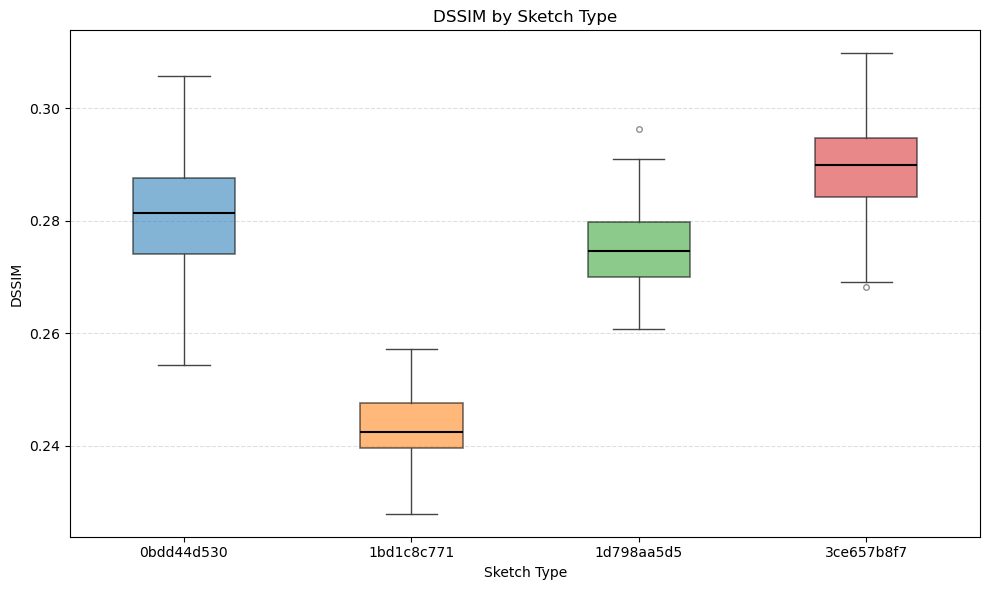
\includegraphics[width=1\linewidth]{images/boxplots}
	\caption{Box plot of DSSIM values for sketches groups}
	\label{fig:boxplots}
\end{figure}


\begin{table*}[htbp]
	\centering
    \sisetup{output-decimal-marker = {.}}
	\caption{Summary statistics for MSE, DSSIM, and LBP Distance across four groups and total.}
	\label{tab:metricsSummary}
	\begin{tabular*}{\textwidth}{@{\extracolsep{\fill}}l S[table-format=4.2] S[table-format=4.2] S[table-format=4.2] S[table-format=4.2] S[table-format=4.2]@{}}
		\toprule
		& {\textbf{Group 1}} & {\textbf{Group 2}} & {\textbf{Group 3}} & {\textbf{Group 4}} & {\textbf{Total}} \\
		\midrule
		\multicolumn{6}{c}{\textbf{MSE}} \\
		\midrule
		Min    & 718.12  & 651.21 & 511.83 & 987.74  & 511.83 \\
		Q1     & 855.92  & 686.99 & 535.13 & 1056.76 & 643.62 \\
		Median & 916.33  & 718.47 & 542.87 & 1093.89 & 779.19 \\
		Q3     & 963.64  & 740.92 & 556.09 & 1127.13 & 1005.90 \\
		Max    & 1098.81 & 794.37 & 620.87 & 1202.46 & 1202.46 \\
		\midrule
		\multicolumn{6}{c}{\textbf{DSSIM}} \\
		\midrule
		Min    & 0.2544 & 0.2279 & 0.2608 & 0.2683 & 0.2279 \\
		Q1     & 0.2741 & 0.2395 & 0.2701 & 0.2842 & 0.2567 \\
		Median & 0.2814 & 0.2424 & 0.2746 & 0.2900 & 0.2766 \\
		Q3     & 0.2876 & 0.2475 & 0.2798 & 0.2947 & 0.2870 \\
		Max    & 0.3057 & 0.2572 & 0.2963 & 0.3098 & 0.3098 \\
		\midrule
		\multicolumn{6}{c}{\textbf{LBP - DISTANCE}} \\
		\midrule
		Min    & 0.0800 & 0.1200 & 0.0400 & 0.1900 & 0.0400 \\
		Q1     & 0.1500 & 0.1300 & 0.0700 & 0.2200 & 0.1043 \\
		Median & 0.2000 & 0.1500 & 0.0800 & 0.2300 & 0.1640 \\
		Q3     & 0.2500 & 0.1700 & 0.0900 & 0.2400 & 0.2215 \\
		Max    & 0.3900 & 0.2000 & 0.1100 & 0.2700 & 0.3900 \\
		\bottomrule
	\end{tabular*}
\end{table*}
\section{Ablation Study}
\label{sec:ablation}

\PARstart{T}{o} assess the contribution of each component of our proposed methodology, we suggest a series of ablation studies. We design these experiments to isolate the impact of the VAE-based context generation and the context-oriented texture synthesis on the final quality of the synthetic images.

\subsection{Impact of Context-Oriented Synthesis}

A key innovation of our method is the division of the synthesis process into three distinct zones: salt, conventional rock, and their boundary. To evaluate the importance of this separation, we propose an experiment where this context-oriented approach is removed.

\begin{itemize}
    \item \textbf{Experiment}: A single, non-parametric texture synthesis model would be used to generate the entire image, guided only by the binary salt/non-salt mask produced by the VAE. This model would not differentiate between the interior of the salt dome, the surrounding rock, and the crucial boundary region.
    \item \textbf{Hypothesis}: We expect a significant degradation in image quality. The model would likely struggle to reproduce the sharp, geologically complex interfaces between salt and sediment, resulting in blurred or unrealistic boundaries.
    \item \textbf{Evaluation}: The results would be compared against our full method using the same quantitative metrics (MSE, DSSIM, LBP Distance) and qualitative expert analysis. A poorer performance would validate the necessity of our context-oriented approach.
\end{itemize}

\subsection{Contribution of the VAE for Mask Generation}

Our method relies on a VAE to generate realistic and diverse salt body geometries. An ablation study could quantify the benefit of this component compared to simpler alternatives.

\begin{itemize}
    \item \textbf{Experiment}: Replace the VAE with a more basic mask generation technique. For instance, new masks could be created by applying simple geometric transformations (e.g., rotation, scaling, elastic deformation) to the existing ground-truth masks from the training set.
    \item \textbf{Hypothesis}: While simpler, this approach would likely yield a less diverse and geologically plausible set of masks. We hypothesize that the VAE's ability to learn a rich latent distribution of salt geometries is crucial for generating high-quality and varied synthetic samples.
    \item \textbf{Evaluation}: The quality of the final synthetic images generated using these simpler masks would be assessed. A lower score in expert evaluations and quantitative metrics would underscore the VAE's contribution to the realism and diversity of the augmented dataset.
\end{itemize}

\subsection{Relevance of Boundary-Specific Synthesis}

The proposed method gives special treatment to the boundary zone, using patch selection oriented by local angles to construct the interface. The importance of this specific step can be evaluated as follows:

\begin{itemize}
    \item \textbf{Experiment}: We would disable the angle-aware patch selection for the boundary zone. We would synthesize the boundary using the same standard non-parametric texture synthesis applied to the salt and rock interiors, without considering the local orientation of the interface.
    \item \textbf{Hypothesis}: We predict that this change would lead to less coherent and realistic boundaries. We would lose the fine-grained textural details that align with the curve of the salt dome, resulting in visible artifacts and a less convincing transition between the geological layers.
    \item \textbf{Evaluation}: A direct comparison of the boundary regions between this ablated version and the full model, both qualitatively by experts and quantitatively (if a suitable metric for boundary coherence is defined), would highlight the value of this specialized synthesis step.
\end{itemize}

These proposed studies would systematically validate our design choices and provide a deeper understanding of why the proposed context-oriented approach is effective for synthesizing high-fidelity seismic images.
\section{Conclusions and Future Work}
\label{sec:conclusion}

\PARstart{T}{his} work proposed a data augmentation scheme based on the context-oriented synthetic generation of seismic image data containing salt bodies, since such imagery data can be relevant for training robust seismic image analysis methods for prospecting petroleum in deep waters. The proposed scheme combines a deep neural network model with non-parametric synthesis. The experimental results, using the TGS-Dataset as input, suggest that the proposed methodology can be potentially effective for generating seismic imagery data containing salt bodies, as indicated by the evaluation conducted by experts in the field. The results show similar measures of precision, recall, and F1-scores for both the real and the synthesized seismic image data. 

The synthetic samples potentially can be used in geological studies and situations where real data may be scarce or unavailable. The close resemblance between synthetic and real images suggests that the synthesized datasets may be used in geoscience research.

As future work, we plan to test the proposed method in other datasets to assess the resilience of the proposed methodology and to evaluate the benefit of training smart seismic image segmentation schemes using the synthesized seismic images as data augmentation.


\begin{thebibliography}{00}

\bibitem{Zeng2019}
Y.~Zeng, K.~Jiang, and J.~Chen, ``Automatic seismic salt interpretation with deep convolutional neural networks,'' in \emph{Int. Conf. Inf. Syst. Data Min. - ICISDM 2019}, 2019, pp. 16--20, doi: 10.1145/3325917.3325926.

\bibitem{He2016}
K.~He, X.~Zhang, S.~Ren, and J.~Sun, ``Deep residual learning for image recognition,'' in \emph{2016 IEEE Conference on Computer Vision and Pattern Recognition (CVPR)}, 2016, pp. 770--778, doi: 10.1109/CVPR.2016.90.

\bibitem{Ronneberger2015}
O.~Ronneberger, P.~Fischer, and T.~Brox, ``U-Net: Convolutional networks for biomedical image segmentation,'' in \emph{Medical Image Computing and Computer-Assisted Intervention -- MICCAI 2015}, 2015, pp. 234--241.

\bibitem{Henriques2021}
L.~Henriques, S.~Colcher, R.~Milidiú, A.~Bulcão, and P.~Barros, ``Generating data augmentation samples for semantic segmentation of salt bodies in a synthetic seismic image dataset,'' arXiv, Jun. 2021. [Online]. Available: http://arxiv.org/abs/2106.08269

\bibitem{Li2020}
K.~Li, S.~Chen, and G.~Hu, ``Seismic labeled data expansion using variational autoencoders,'' \emph{Artif. Intell. Geosci.}, vol. 1, pp. 24--30, Dec. 2020, doi: 10.1016/j.aiig.2020.12.002.

\bibitem{Gatys2015}
L.~Gatys, A.~S.~Ecker, and M.~Bethge, ``Texture synthesis using convolutional neural networks,'' in \emph{Advances in Neural Information Processing Systems}, Curran Associates, Inc., 2015.

\bibitem{Zhou2018}
Y.~Zhou, Z.~Zhu, X.~Bai, D.~Lischinski, D.~Cohen-Or, and H.~Huang, ``Non-stationary texture synthesis by adversarial expansion,'' \emph{ACM Trans. Graph.}, vol. 37, no. 4, pp. 49:1--49:13, Jul. 2018, doi: 10.1145/3197517.3201285.

\bibitem{Powers2011}
D.~M.~W.~Powers, ``Evaluation: From precision, recall and F-measure to ROC, informedness, markedness \& correlation,'' \emph{Journal of Machine Learning Technologies}, 2011.

\bibitem{Kingma2014}
D.~P.~Kingma and M.~Welling, ``Auto-encoding variational Bayes,'' arXiv, May 2014, doi: 10.48550/arXiv.1312.6114.

\bibitem{Efros1999}
A.~A.~Efros and T.~K.~Leung, ``Texture synthesis by non-parametric sampling,'' in \emph{Proceedings of the Seventh IEEE International Conference on Computer Vision}, Kerkyra, Greece, 1999, vol. 2, pp. 1033--1038, doi: 10.1109/ICCV.1999.790383.

\bibitem{Wang2021}
T.~Wang, D.~Trugman, and Y.~Lin, ``SeismoGen: Seismic waveform synthesis using GAN with application to seismic data augmentation,'' \emph{Journal of Geophysical Research: Solid Earth}, vol. 126, no. 4, p. e2020JB020077, 2021, doi: 10.1029/2020JB020077.

\bibitem{Anjom2024}
F.~Khosro Anjom, F.~Vaccarino, and L.~V.~Socco, ``Machine learning for seismic exploration: Where are we and how far are we from the holy grail?'' \emph{GEOPHYSICS}, vol. 89, no. 1, pp. WA157--WA178, Jan. 2024, doi: 10.1190/geo2023-0129.1.

\bibitem{Choi2025}
B.~Choi, S.~Pyun, W.~Choi, and Y.~Cho, ``Synthetic seismic data generation with pix2pix for enhanced fault detection model training,'' \emph{Computers \& Geosciences}, vol. 197, p. 105879, Mar. 2025, doi: 10.1016/j.cageo.2025.105879.

\bibitem{Zhou2024}
Y.~Zhou, R.~Xiao, D.~Lischinski, D.~Cohen-Or, and H.~Huang, ``Generating non-stationary textures using self-rectification,'' in \emph{Proceedings of the IEEE/CVF Conference on Computer Vision and Pattern Recognition}, 2024, pp. 7767--7776.

\bibitem{TGS2023}
TGS Kaggle, ``TGS Salt Identification Challenge | Kaggle,'' 2023. [Online]. Available: https://www.kaggle.com/competitions/tgs-salt-identification-challenge/data

\bibitem{Ferreira2020}
R.~S.~Ferreira, J.~Noce, D.~A.~B.~Oliveira, and E.~V.~Brazil, ``Generating sketch-based synthetic seismic images with generative adversarial networks,'' \emph{IEEE Geoscience and Remote Sensing Letters}, vol. 17, no. 8, pp. 1460--1464, Aug. 2020, doi: 10.1109/LGRS.2019.2945680.

\bibitem{Vatamanu2013}
O.~A.~Vatamanu, M.~Frandes, M.~Ionescu, and S.~Apostol, ``Content-based image retrieval using local binary pattern, intensity histogram and color coherence vector,'' in \emph{2013 E-Health and Bioengineering Conference (EHB)}, Nov. 2013, pp. 1--6, doi: 10.1109/EHB.2013.6707396.

\bibitem{BrittoMattos2017}
A.~Britto Mattos, R.~S.~Ferreira, R.~M.~Da Gama e Silva, M.~Riva, and E.~V.~Brazil, ``Assessing texture descriptors for seismic image retrieval,'' in \emph{2017 30th SIBGRAPI Conference on Graphics, Patterns and Images (SIBGRAPI)}, Oct. 2017, pp. 292--299, doi: 10.1109/SIBGRAPI.2017.45.

\end{thebibliography}

\begin{IEEEbiography}[{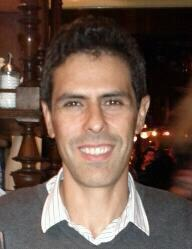
\includegraphics[width=1in,height=1.25in, clip,keepaspectratio]{images/luciano.jpg}}]{Luciano D. Terres}
Received the B.S. degree in Computer Science from the Federal University of Rio
Grande do Sul (UFRGS), Brazil, in 1996. In 2010 received the M.S. degree in
Engineering and Computer Systems from the Federal University of Rio de Janeiro (UFRJ-COPPE), Brazil.
Currently, he is a Ph.D. student in Computer Science at UFRGS. Since 2005 has been a researcher at Petrobras Cenpes Research Center.
His research interests include petroleum exploration, petroleum systems simulation, computer vision, image processing, and pattern recognition.

\end{IEEEbiography}

\begin{IEEEbiography}[{\includegraphics
[width=1in,height=1.25in,clip,
keepaspectratio]{images/jacob.jpg}}]
{Jacob Scharcanski}
received the B.Sc. degree in electrical engineering in 1981 and the M.Sc.
degree in computer science in 1987, both from the Federal University of Rio
Grande do Sul (UFRGS), Brazil, and the Ph.D. degree in systems design
engineering from the University of Waterloo, Canada, in 1993. Currently, he
is a Full Professor in computer science at UFRGS.  He has authored and
co-authored over 170 refereed journal and conference papers, and has
contributed to several books on imaging and measurements. In addition to his
academic publications, he has several technology transfers to the private
sector. Presently, he serves as an Associate Editor for two journals and has
served on dozens of International Conference Committees. Prof. Scharcanski is
a Senior Member of the IEEE, and served as an IEEE IMS Distinguished Lecturer
on several occasions. His areas of expertise are Image Processing, Pattern
Recognition, Imaging Measurements and Computational Methods in Finance.
\end{IEEEbiography}

\EOD
\end{document}
